\documentclass[aspectratio=169,t,11pt,table]{beamer}
\usepackage{../../slides,../../math}
\definecolor{accent}{HTML}{2B5269}
\definecolor{accent2}{HTML}{9D2235}

\title{Topic 3: Selection on Observables}
\subtitle{\it  ECON 5783 — University of Arkansas}
\date{Fall 2024}
\author{Prof. Kyle Butts}

\begin{document}

% ------------------------------------------------------------------------------
\begin{frame}[noframenumbering,plain]
\maketitle

% \bottomleft{\footnotesize $^*$A bit of extra info here. Add an asterich to title or author}
\end{frame}
% ------------------------------------------------------------------------------

\section{Conditional Independence Assumption}

\begin{frame}{Selection into Treatment}
  In our last lectures, we have covered the problem with difference-in-means comparisons:
  \begin{itemize}
    \item If units with $D_i = 1$ have different characteristics on average than units with $D_i = 0$, then we are making faulty comparisons
  \end{itemize}

  \pause
  \bigskip
  In the absence of treatment, the control units and the treated units would have different average $Y_i(0)$ due to differences in characteristics
\end{frame}

\begin{frame}{Selection into Treatment and Omitted Variable Bias}
  We have shown that if there is a single problematic covariate, $X_2$, that differs between the treated group and control group, our difference-in-means estimator is biased:
  \begin{align*}
    \hat{\tau}_{\text{DIM}} &= 
    \expec{Y_{i}}{D_i = 1} - \expec{Y_{i}}{D_i = 0} \\
    &= \tau_{\text{ATT}} + \frac{\beta_2}{1 - \prob{D = 1}} \left( \expec{X_2}{D = 1} - \expec{X_2} \right)
  \end{align*}

  \pause
  \begin{itemize}
    \item The ATT estimate reflects the impact that differences in $X_2$ have on the outcome $\beta_2$
  \end{itemize}
\end{frame}

\begin{frame}{Controls}
  This raises the simple question: what if we compare treated and control units with the same values of $X_2$?
  \begin{itemize}
    \item Subset the control units to those that ``look like'' the treated units
  \end{itemize}

  \pause
  \bigskip
  This is a reasonable strategy in some settings and understanding it is the goal of this topic
\end{frame}

\begin{frame}{Conditional Independence Assumption}
  The \alert{Conditional Independence Assumption} is given by
  $$
    (Y_{i}(0), Y_{i}(1)) \Perp D_i \ \vert \ \bm{X}_i
  $$
  \begin{itemize}
    \item This says that for units with the same value of $\bm{X}_i = \bm{x}$, treatment is independent of the potential outcomes (i.e. ``randomly assigned'')
  \end{itemize}

  \pause
  \bigskip
  This is like a randomized control trial except you can only compare treated and control units with the same $\bm{X}_i$
\end{frame}

\begin{frame}{Example 1}{Effect of attending a prestiguous school}
  Dale and Krueger (2002, QJE) estimate the effect of attending a more selective college on future earnings
  \begin{itemize}
    \item Whether or not you get accepted into a more selective college is not randomly assigned
  \end{itemize}

  \pause
  \bigskip
  Using data on the full list of schools that students were accepted to, they argue that for students who got into the same schools, whether they went to the more selective college is random (independent of potential outcomes)
\end{frame}

\begin{frame}{Example 2}{Winning the Lottery}
  Imbens, Rubin, and Sacerdote (2001, AER) estimate the impact of unearned income on labor supply using the lottery
  \begin{itemize}
    \item While winning the lottery is random \emph{among those that play}, playing the lottery is not randomly assigned. 
    
    \item Even among players, some play more frequently
    
    \item Comparing lottery winners labor supply to the population would be biased since lottery \emph{players look different}
  \end{itemize}
  
  \pause
  \bigskip
  They argue that conditional on playing and winning in the lottery ($X_i$), winning a small amount (control) or a large amount (treatment) is randomly assigned
\end{frame}

\begin{frame}{Example 3}{Charter Schools}
  Abdulkadiroğlu, Angrist, and Pathak (2014, ECTA) estimate the impact of attending an elite ``exam school'' in NYC on students' success.
  \begin{itemize}
    \item These schools accept students with very high scores on a centralized exam
  \end{itemize}

  \pause
  \bigskip
  However, these schools are over-subscribed to and have to create admission cutoffs 
  \begin{itemize}
    \item Compare students just on either end of the cutoff score. Since the test scores are likely noisy, these students are randomly assigned to the best schools or slightly lower quality schools
  \end{itemize}
\end{frame}

% \begin{frame}{Example 3}{Charter Schools}
%   Abdulkadiroğlu, Angrist, Dynarski, Kane, and Pathak (2011, QJE) use Boston charter school over-application and offer lotteries to estimate the impact of Charter Schools
%   \begin{itemize}
%     \item Which charter that a student applied
%   \end{itemize}
% \end{frame}

\begin{frame}{Example 4}{College Athletic Success}
  Anderson (2017, RESTAT) estimates the effect of having a successful college athletics program help colleges (say recruit better students)

  \begin{itemize}
    \item Whether or not a school is good at athletics is not randomly assigned
  \end{itemize}
  
  Uses gambling bookmakers' ``spreads'' as a measure of predicted odds of a school winning (in football) games. They compare schools with the same odds of winning; those that won more than expected to those that won fewer
\end{frame}

\begin{frame}{Example 5}{Macroeconomic Policy Shocks}
  Angrist, Jordà, and Kuersteiner (2016, JASA) estimate the impact of unexpected changes to intereste rates on the economy

  \begin{itemize}
    \item The Fed makes decisions on interest rates based on economic conditions (reverse causality)
  \end{itemize}

  The prices of conracts in the futures markets reflect the \emph{expected} change in interest rates, so they compare interest rate changes with the same expected change but different unexpected changes
\end{frame}


\begin{frame}{Block-randomized Experiments}
  Say you run an experiment where you assign treatment to men randomly with probability 25\% and to women randomly with probability 75\%. 
  \begin{itemize}
    \item By randomization, we have $ (Y_{i}(0), Y_{i}(1)) \Perp D_i \ \vert \ F_i$ where $F_i$ is an indicator for being a female
  \end{itemize}

  \pause
  \bigskip
  Say $\expec{Y_i(0)}{F_i = 1} \neq \expec{Y_i(0)}{F_i = 0}$. 
  \begin{itemize}
    \item Then since treatment is correlated with gender, $Y_{i}(0) \not\Perp D_i$. Even though we randomize for each gender, we do not have (unconditional) independence
  \end{itemize}
\end{frame}

\begin{frame}{Clustered Experiments}
  Our differnece-in-means estimator using the whole population will be biased.
  \begin{itemize}
    \item However, doing difference-in-means separately for male and femals is valid (conditional independence holds!)
  \end{itemize}

  \bigskip
  What does each difference-in-means estimator estimate?
\end{frame}

\begin{frame}{Clustered Experiments}
  What does each difference-in-means estimator estimate? Under conditional independence
  \begin{align*}
    \tau_{\text{DIM},\text{Female}} 
    &= \expec{Y_{i}}{D_i = 1, F_i = 1} - \expec{Y_{i}}{D_i = 0, F_i = 1}  \\ \pause
    &= \expec{Y_{i}(1) - Y_{i}(0)}{F_i = 1} = \tau(F_i = 1)
  \end{align*}

  \bigskip 
  We estimate the conditional average treatment effect by gender!
\end{frame}

\begin{frame}{Clustered Experiments}
  How do we estimate the overall average treatment effect? 
  \begin{align*}
    \tau_{\text{ATE}} &= \expec{\tau_i} = \expec{\tau(F_i)} \\
    &= \tau(F_i = 1) * \prob{F_i = 1} + \tau(F_i = 0) \prob{F_i = 0}
  \end{align*}
  \begin{itemize}
    \item Weighted average of the CATE with weights proportional to group size
  \end{itemize}
\end{frame}

\begin{frame}{Generalization}
  In more general settings where $\bm{X}_i$ is (possibly) continuous and multi-dimensional, we can still do the same procedure:
  \begin{itemize}
    \item For each value of $\bm{x}$, calculate difference in means of treated and control units with $\bm{X}_i = \bm{x}$
    
    \item Integrate (average) the difference-in-means estiamtes using the distribution of $X$ 
  \end{itemize}

  \pause
  \vspace*{-\medskipamount}
  \begin{align*}
    \tau_{\texttt{ATE}} &= 
    \int_{\bm{x} \in \mathbb{X}} \tau(\bm{X}_i = \bm{x}) d\prob{\bm{X} = \bm{x}} \\ 
    &= \int_{\bm{x} \in \mathbb{X}} \expec{Y_i}{D_i = 1, \bm{X}_i = \bm{x}} - \expec{Y_i}{D_i = 0, \bm{X}_i = \bm{x}} d\prob{\bm{X} = \bm{x}}
  \end{align*}
\end{frame}

\begin{frame}{Generalization}
  If we want the average treatment effect on the treated, we average over the distribution of $\bm{X}$ for the treated group
  
  \vspace*{-\medskipamount}
  \begin{align*}
    \tau_{\text{ATT}} &= 
    \int_{\bm{x} \in \mathbb{X}} \tau(\bm{X}_i = \bm{x}) d\prob{\bm{X} = \bm{x}}{D_i = 1}\\ 
    &= \int_{\bm{x} \in \mathbb{X}} \expec{Y_i}{D_i = 1, \bm{X}_i = \bm{x}} - \expec{Y_i}{D_i = 0, \bm{X}_i = \bm{x}} d\prob{\bm{X} = \bm{x}}{D_i = 1}
  \end{align*}
\end{frame}

\begin{frame}{Example 2}{Attending College}
  Say we want to know the effect of college on future earnings in an observational study. 
  
  \bigskip
  We might not believe that attending college $D_i$ is randomly assigned to workers
  \begin{itemize}
    \item But we might think that for workers with the same high-school GPA, same family income, and same parental education status ($\bm{X}_i$), whether or not a worker attends college is independent of outcomes
  \end{itemize}
\end{frame}

\begin{frame}{What drives treatment after conditioning on $\bm{X}_i$}
  To be clear, \emph{something} must be causing some units to sign up for treatment and others not to
  \begin{itemize}
    \item Maybe some teacher encouraged person A to apply but person B was not 
    \begin{itemize}
      \item Since this is probably unrelated to future earnings, this is in support of conditional independence assumption
    \end{itemize}
    
    \pause
    \item Or maybe how many college-going classmates you impacts whether or not you go
    \begin{itemize}
      \item Since these peer effects probably impact future earnings, this is in not in support of conditional independence assumption
    \end{itemize}
  \end{itemize}
\end{frame}

\begin{frame}{Using this method}
  There is always going to be debate with this method on what variables are missing in $\bm{X}_i$
\end{frame}

\imageframe{figures/pt1.png}
\imageframe{figures/pt2.png}

\begin{frame}{Using this method}
  There is always going to be debate with this method on what variables are missing in $\bm{X}_i$
  \begin{itemize}
    \item Author: ``$\bm{X}_i$ includes a lot of important factors that drive selection into treatment!''
    \item Reviewer: ``I think there are other omitted variables that drive selection into treatment!!''
  \end{itemize}

  \bigskip
  I think this is one reason why this method is not more popular; your luck in publishing depends on whether or not your referee ``believes'' you have included the right variables in $\bm{X}_i$
\end{frame}

\begin{frame}{Military Service and Future Earnings}
  Angrist (1998) studies how military service affects future earnings
  \begin{itemize}
    \item Non-random selection into volunteering for the military
    \item Matches on $\bm{X} = $ race, application year, years of schooling, Armed Forces Qualification Test score group, and year of birth
  \end{itemize}

  \bigskip
  Compares each veteran to a non-veteran worker with the same exact charactersitics
  \pause
  \begin{itemize}
    \item Might not be perfect, but does a better job at alleviating concerns about selection into treatment
    \item I think the AFQT score helps quite a bit
  \end{itemize}
\end{frame}

\begin{frame}{Why selection on observables is hard}{Evictions}
  Collinson, Humphries, Mader, Reed, Tannenbaum, and Van Dijk (2023, QJE) study the effect of being evicted on future earnings

  \bigskip
  Eviction courts randomly assign cases to judges of varying `leniency'
  \begin{itemize}
    \item Some are assigned to harsh judges while others are assigned to more lenient ones
  \end{itemize}
\end{frame}

\begin{frame}{Why selection on observables is hard}{Evictions}
  They first perform an analysis like previous work in the literature:
  \begin{itemize}
    \item Compare evicted and non-evicted individuals of similar demographics: e.g. income, race, highest level of education, gender, marital status,
    children, age, past criminal record, past job loss, past relationship dissolution, and housing assistance receipt
  \end{itemize}
  
  \bigskip
  They find large and significant effects on earnings
\end{frame}

\begin{frame}{Why selection on observables is hard}{Evictions}
  Second, they show using adminsitrative data on credit-scores, that even conditional on those demographic characteristcs, those that get eviced have sharp declines in earnings just prior to eviction
  \begin{itemize}
    \item The evicted people likely would have worse $Y(0)$ (in the absence of eviction) than those that were not evicted
  \end{itemize}

  \pause
  \bigskip
  Results are still negative, but significantly smaller
  \begin{itemize}
    \item Even though the observables that previous work has matched on were quite `rich', there was still a large role for unobservables
  \end{itemize}
\end{frame}

% \begin{frame}{}
%   Aizer and Doyle (2015, QJE)  find similar dynamics with teenages and crime courts
% \end{frame}


\section{Regression Adjustment}

\begin{frame}{Reminder of Setup}
  We observe a sample of $n$ observations, $Y$ is outcome, $\bm{X}$ is a vector of control variables, $D$ is our treatment variable of interest. We assume the conditional independence assumption
  $$
    (Y_{i}(0), Y_{i}(1)) \Perp D_i \ \vert \ \bm{X}_i = \bm{x}
  $$

  \pause
  \bigskip
  Our average-treatment effect estimate can be written as the average of CATE (averaged over distribution of $X$)
  $$
    \tau_{\texttt{ATE}} = \expec{\ \expec{Y_i(1)}{\bm{X}_i} - \expec{Y_i(0)}{\bm{X}_i} \ }
  $$
\end{frame}

\begin{frame}{Conditional Expectation Function}
  $$
  \tau_{\texttt{ATE}} = \expec{\ \expec{Y_i(1)}{\bm{X}_i} - \expec{Y_i(0)}{\bm{X}_i} \ }
  $$

  There are two conditional expectation functions in the above terms. Define
  $$
    \mu_0(\bm{x}) = \expec{Y_i(0)}{\bm{X}_i = \bm{x}} 
    \text{ and }
    \mu_1(\bm{x}) = \expec{Y_i(1)}{\bm{X}_i = \bm{x}}
  $$

  \pause
  \bigskip
  Then, the above becomes $\tau_{\texttt{ATE}} = \expec{ \mu_1(\bm{X}_i) - \mu_0(\bm{X}_i) }$
  \begin{itemize}
    \item If we knew the CEF, then we can estimate this with $\frac{1}{n} \sum_{i=1}^n \mu_1(\bm{X}_i) - \mu_0(\bm{X}_i)$
  \end{itemize}
\end{frame}

\begin{frame}{Estimation of the conditional expectation functions}
  \vspace*{-\bigskipamount}
  $$
    \mu_0(\bm{x}) = \expec{Y_i(0)}{\bm{X}_i = \bm{x}} 
    \text{ and }
    \mu_1(\bm{x}) = \expec{Y_i(1)}{\bm{X}_i = \bm{x}}
  $$

  \bigskip
  Since we have conditional independence assumption: 
  $$
    \expec{Y_i(0)}{\bm{X}_i = \bm{x}, D_i = 0} = \expec{Y_i(0)}{\bm{X}_i = \bm{x}} = \mu_0(\bm{x})
  $$ 
  \begin{itemize}
    \item We can estimate $\mu_0(\cdot)$ and $\mu_1(\cdot)$ using the untreated and treated group, respectively

    \item We have talked about many different ways to estimate the CEF (e.g. linear regression)
  \end{itemize}
\end{frame}

\begin{frame}{Linear model for CEF}
  Say we estimate $\mu_0(\bm{x})$ and $\mu_1(\bm{x})$ using linear regressions of $Y$ on $\bm{X}$ for the untreated and treated groups respectively:
  $$
    Y_i = \alpha_{d} + \bm{X}_{i}' \beta_d + u_{id}
  $$
  \begin{itemize}
    \item The control-sample regression gives us $\hat{\alpha}_{0}$, $\hat{\beta}_{0}$ and the treated-sample regression gives us $\hat{\alpha}_{1}$, $\hat{\beta}_{1}$
  \end{itemize}
\end{frame}

\begin{frame}{Regression Adjustment}{\texttt{ATE} Estimator}
  The \alert{regression adjustment treatment effect estimators} are given by:
  $$
    \hat{\tau}_{\texttt{ATE}} = 
    \underbrace{
      \frac{1}{n} \sum_{i=1}^n \left( \hat{\alpha}_1 + \bm{X}_i' \hat{\beta}_1 \right)
    }_{\expechat{Y_i(1)}} -
    \underbrace{
      \frac{1}{n} \sum_{i=1}^n \left( \hat{\alpha}_0 + \bm{X}_i' \hat{\beta}_0 \right)
    }_{\expechat{Y_i(0)}} 
  $$
  \begin{itemize}
    \item Predicting everyone's $Y_i(1)$ and $Y_i(0)$ given their $\bm{X}_i$ and taking the difference
    \item Quality of estimator therefore depends on quality of conditional expectation model
  \end{itemize}
\end{frame}

\begin{frame}{Regression Adjustment}{\text{ATT} Estimator}
  $$
    \hat{\tau}_{\text{ATT}} = 
    \underbrace{
      \frac{1}{n_1} \sum_{i=1}^n D_i \left( \hat{\alpha}_1 + \bm{X}_i' \hat{\beta}_1 \right)
    }_{\expechat{Y_i(1)}{D_i = 1}} - 
    \underbrace{
      \frac{1}{n_1} \sum_{i=1}^n D_i \left( \hat{\alpha}_0 + \bm{X}_i' \hat{\beta}_0 \right)
    }_{\expechat{Y_i(0)}{D_i = 1}} 
  $$
\end{frame}

\begin{frame}{Regression Adjustment}
  For the \text{ATT}, remember that the fitted value of a linear regression averaged over the estimation sample is the average of $Y$ for that sample.
  
  \bigskip
  So, we can rewrite the 
  \begin{align*}
    \hat{\tau}_{\text{ATT}} &= 
    \frac{1}{n_1} \sum_{i=1}^n D_i \left( \hat{\alpha}_1 + \bm{X}_i' \hat{\beta}_1 \right) -
    \frac{1}{n_1} \sum_{i=1}^n D_i \left( \hat{\alpha}_0 + \bm{X}_i' \hat{\beta}_0 \right) \\ 
    &= \frac{1}{n_1} \sum_{i=1}^n D_i Y_i - 
    \frac{1}{n_1} \sum_{i=1}^n D_i \left( \hat{\alpha}_0 + \bm{X}_i' \hat{\beta}_0 \right) 
  \end{align*}
  \begin{itemize}
    \item Only relying on the model for $\mu_{0}(\bm{x})$ to estimate the \text{ATT}
  \end{itemize}
\end{frame}

\begin{frame}{Regression Adjustment via Regression}
  You can force regression to estimate this for you in a single regression; this makes producing valid standard errors easier
  $$
    Y_i = \alpha_0 + \alpha_1 D_i + \beta_0 \bm{X}_i + \beta_1 D_i * (\bm{X}_i - \bar{\bm{X}}) + u_i
  $$
  \begin{itemize}
    \item Then our $\hat{\tau}_{\texttt{ATE}}$ estimate is given by $\hat{\alpha}_1$
    \item If you subtract of the average of $\bm{X}$ for the treated group, $\hat{\alpha}_1$ will be $\hat{\tau}_{\text{ATT}}$
  \end{itemize}
\end{frame}

\begin{frame}{Coding implementation}
  In \texttt{R}, use the \texttt{fixest} package to estimate the regression with \texttt{HC1} standard errors

  \bigskip
  In \texttt{Stata}, use the \texttt{teffects ra} command
\end{frame}

\begin{frame}{Function form of CEF Models}
  The main difficulty with this estimator is that we need to be confident in our model of $\mu_d(\bm{x}) = \expec{Y_i(d)}{\bm{X}_i = \bm{x}}$
  \begin{itemize}
    \item Can do better if we include polynomials of or bin continuous variables 
    \item Set of indicators for discrete varaibles
    \item Consider important interactions between variables
  \end{itemize}

  \bigskip
  See Imbens and Wooldridge (2009, JEL) review article for more details
\end{frame}

\begin{frame}{Regression Adjustment in RCTs}
  When treatment is completely randomly assigned, covariates are balanced \emph{on average}
  \begin{itemize}
    \item For a single draw of the experiment, some covariates may remain unbalanced
  \end{itemize}

  \pause
  \bigskip
  It is often common practice to show the difference-in-means estimator and a second regression-adjustment estimate
  \begin{itemize}
    \item Lin (2013) and Nagi and Wooldridge (2021) show that the latter improves efficiency even in an RCT
  \end{itemize}
\end{frame}

\section{Matching estimators}

\begin{frame}{Curse of dimensionality strikes again!}
  Given the conditional independence assumption (CIA), 
  $$
    (Y_{i}(0), Y_{i}(1)) \Perp D_i \ \vert \ \bm{X}_i
  $$
  we can theoretically perform a bunch of different difference-in-means estimators and then aggregate covariate-specific estimates
  \begin{itemize}
    \item This works well when $X_i$ is a single binary variable
  \end{itemize}

  \pause
  \bigskip
  But as we add more and more covariates, the fewer observations we have for $\bm{X}_i = \bm{x}$
  \begin{itemize}
    \item What do we do if there are no treated units or no control units for a given $\bm{x}$?
  \end{itemize}
\end{frame}

\begin{frame}{Finding comparable control units}
  \begin{center}
    What do we do if there are no treated units or no control units for a given $\bm{x}$?
  \end{center}

  \bigskip
  One strategy we could take is to find a control unit for each treated unit that has an $\bm{X}_i$ that is ``close'' to a given treated unit's $\bm{x}$
  \begin{itemize}
    \item For each treated unit $i$, find a matching control unit (or units), $j$, that has $\bm{X}_i \approx \bm{X}_j$
  \end{itemize}
\end{frame}

\begin{frame}{Matching estimator}
  Let $j(i)$ be the unit that is matched to treated unit $i$. Let $N_1 = \sum_i D_i$ be the number of treated units. 
  
  \bigskip 
  Our treatment effect estimator is given by:
  $$
    \hat{\tau}_{\text{Matching}}
    \underbrace{\frac{1}{N_1} \sum_{i = 1}^n D_i Y_i}_{\text{Treated group average}} -
    \underbrace{\frac{1}{N_1} \sum_{i = 1}^n D_i Y_{j(i)}}_{\text{Matched control group average}}
  $$
\end{frame}

\begin{frame}{Matching estimator}
  $$
    \expechat{Y_i(0)}{D_i = 1} = \frac{1}{N_1} \sum_{i = 1}^n D_i Y_{j(i)}
  $$

  \bigskip
  Each control unit has (approximately) the same $\bm{X}$ as it's respective treated unit so their $Y(0)$ is a good estimate (on average) for the treated unit's $Y(0)$.
    
  \pause
  \bigskip
  The matched control units $\{ j(i): D_i = 1 \}$ have the same distribution of $\bm{X}$ as the treated units (by design), so in some sense you are removing selection on $\bm{X}$
\end{frame}

\begin{frame}{Defining ``close''}
  How do we decide which control units are close? We need some measure of ``distance''. 

  \bigskip
  The simplest measure is the \alert{euclidean distance}. For units $i$ and $j$, the distance between $\bm{X}_i$ and $\bm{X}_j$:
  $$
    \sqrt{\sum_{k = 1}^K (X_{i,k} - X_{j, k})^2}
  $$

  \pause 
  \bigskip
  In matrix notation this is 
  $$
    (\bm{X}_i - \bm{X}_j)' (\bm{X}_i - \bm{X}_j)
  $$
\end{frame}

\begin{frame}{Distances}
  $$
    \sqrt{\sum_{k = 1}^K (X_{i,k} - X_{j, k})^2}
  $$

  \bigskip
  Issues with this distance metric:
  \begin{itemize}
    \item Puts more weight on covariates with larger variances (not scale invariant)
    
    \item Each covariate is viewed as being ``equally important to match on''
    
    \item Highly collinear variables get ``counted twice'' in that their discrepencies get summed over twice 
  \end{itemize}

\end{frame}

\begin{frame}{Mahalanobis Distance}
  Can ``scale'' the distances using the variance-covariance matrix of $\bm{X}_i$:
  $$
    S_{\bm{X}\bm{X}'} \equiv \left[ 1/N \sum_{i=1}^N (\bm{X}_i - \bar{\bm{X}}) (\bm{X}_i - \bar{\bm{X}})' \right]
  $$
  \begin{itemize}
    \item The $(k, \ell)$-th element is the sample covariance $\cov{X_{i, k}, X_{i, \ell}}$ and the diagonal being the variance of $X_{i, k}$
    
    \item If the covariance between two elements is high, then we don't want to give ``credit'' to both as ``distinct'' variables
  \end{itemize}
\end{frame}

\begin{frame}{Mahalanobis Distance}
  The \alert{Mahalanobis Distance} is the distance between unit $i$ and $j$'s covariate rescaled by the inverse variance-covariance matrix:
  $$
    (\bm{X}_i - \bm{X}_j)' S_{\bm{X}\bm{X}'}^{-1} (\bm{X}_i - \bm{X}_j)
  $$
  \begin{itemize}
    \item All elements have variance 1 from the rescaling, so this measure is scale-invariant
    
    \item Covariates that are highly collinear do not get counted twice
    
  \end{itemize}
\end{frame}


\begin{frame}{Ensuring we have matches}
  How do we know that there is going to be matchable control units?
  \begin{itemize}
    \item Perhaps units with a certain value (and nearby values) of $\bm{X}_i = x$ are all treated, so there are no (high-quality) controls to match to
  \end{itemize}

  \pause
  \bigskip
  Option 1: We require the \alert{overlap} condition. There is an $\epsilon > 0$ such that for all $x \in \mathbb{X}$
  $$
    1 - \epsilon > \prob{D = 1}{\bm{X} = x} > \epsilon
  $$
  \begin{itemize}
    \item Guarantees that in large samples we will see some treated and control units for each value of $\bm{X}$
  \end{itemize}
\end{frame}

\begin{frame}{Ensuring we have matches}
  Option 2: Subset to treated units that have matchable units
  \begin{itemize}
    \item Changes our definition of the ``population'' and hence our ATT
    
    \item A more subtle point is that if we determine the subsetting based by on our finite sample, then inference gets more complicated
  \end{itemize}
\end{frame}

\begin{frame}{Ensure `balance'}
  It is very common to assess `balance' between covariates after performing matching. 
  \begin{itemize}
    \item Let's the reader verify that the matching is of reasonably high-quality (balance on included $X$s)
    \begin{itemize}
      \item As a reader, don't give too much credit to this (they are trying to match them, so they should be close)
    \end{itemize}
    
    \item Perhaps include other variables that were not included to suggest the treated and matched control group look similar
  \end{itemize}
\end{frame}

\begin{frame}{Ensure `balance'}
  You might be tempted to report a t-test on the difference in means of different $X$ variables between your treated and matched sample
  \begin{itemize}
    \item As your sample size gets larger, you will find significant differences even if they are not \emph{meaningful} differences
  \end{itemize}
  
  \bigskip
  Imbens and Wooldridge (2009, JEL) recommend (as is commonly done) standardized difference-in-means:
  $$
    \frac{\bar{X}_1 - \bar{X}_0}{\sqrt{S_1^2 + S_0^2}}
  $$
  \begin{itemize}
    \item $S_1^2$ and $S_0^2$ are the sample variance of $X$ for the treated and control-group respectively 
  \end{itemize}
\end{frame}

\begin{frame}{Example: Balance Improvements in the Lalonde Data} 
  \begin{table}   
    \footnotesize
    \begin{tabular}{l c c c c c}
      \toprule
      & \multicolumn{2}{c}{\textbf{CPS Controls}} & \multicolumn{2}{c}{\textbf{NSW Treated}} &  \multicolumn{1}{c}{\textbf{Mahalanobis Matched Controls}} \\
      & \multicolumn{2}{c}{(15992)} & \multicolumn{2}{c}{(185)} & (370) \\
      Covariate & mean & (s.d.) & mean & (s.d.) & normalized diff. \\

      \midrule
      Age & 33.23 & (11.05) & 25.82 & (7.16) & -0.16 \\
      Education & 12.03 & (2.87) & 10.35 & (2.01) & -0.09 \\
      Married & 0.71 & (0.45) & 0.19 & (0.39) & -0.20 \\
      Nodegree & 0.30 & (0.46) & 0.71 & (0.46) & 0.18 \\
      Black & 0.07 & (0.26) & 0.84 & (0.36) & 0.00 \\
      Hispanic & 0.07 & (0.26) & 0.06 & (0.24) & 0.00 \\
      Earn '74 & 14.02 & (9.57) & 2.10 & (4.89) & 0.00 \\
      Earn '74 positive & 0.88 & (0.32) & 0.29 & (0.46) & 0.00 \\
      Earn '75 & 13.65 & (9.27) & 1.53 & (3.22) & -0.01 \\
      Earn '75 positive & 0.89 & (0.31) & 0.40 & (0.49) & 0.00 \\
      \bottomrule
    \end{tabular}
  \end{table}
\end{frame}

\begin{frame}{Inference after Matching}
  Note that matching takes on two steps:
  \begin{enumerate}
    \item Create a matched sample using information on $\bm{X}_i$
    \item Estimate a difference-in-means (using regression)
  \end{enumerate}

  The standard errors on the regression estimate ignore the noise generated in step 1
  \begin{itemize}
    \item Incoporating uncertainty from step 1 is a very difficult problem (Guido Imbens and Alberto Abadie, Econometrica 2006)
  \end{itemize}
\end{frame}

\begin{frame}{Coding implementation}
  In \texttt{R}, use the \texttt{MatchIt} package

  \bigskip
  In \texttt{Stata}, use the \texttt{teffects nnmatch} command 
\end{frame}

\section{Propensity-score matching}

\begin{frame}{Reminder of Setup}
  We observe a sample of $n$ observations, $Y$ is outcome, $\bm{X}$ is a vector of control variables, $D$ is our treatment variable of interest. We assume the conditional independence assumption
  $$
    (Y_{i}(0), Y_{i}(1)) \Perp D_i \ \vert \ \bm{X}_i = \bm{x}
  $$

  \pause
  \bigskip
  Our average-treatment effect estimate can be written as the average of CATE (averaged over distribution of $X$)
  $$
    \tau_{\texttt{ATE}} = \expec{\ \expec{Y_i(1)}{\bm{X}_i = \bm{x}} - \expec{Y_i(0)}{\bm{X}_i = \bm{x}} \ }
  $$
\end{frame}

\begin{frame}{Propensity Score}
  Our previous estimator relied on proper modeling of the conditional expectation function. This method, instead, will rely on estimation of the \alert{propensity score} (Rosenbaum and Rubin, 1983):
  $$
    \pi(\bm{x}) = \prob{D_i = 1}{\bm{X}_i = \bm{x}}
  $$
  \begin{itemize}
    \item Looking at units with $\bm{X}_i = \bm{x}$, the propensity score is the probability a random unit in this subset is treated
    \item This was discussed when defining \alert{overlap}: $0 < \pi(\bm{x}) < 1$
  \end{itemize}
\end{frame}

\begin{frame}{Properties of Propensity score}
  Property 1: $\bm{X}$ and $D_i$ are independent conditional on the propensity-score 
  $$
    \bm{X} \Perp D_i \ \vert \ \pi(\bm{X})
  $$
  \begin{itemize}
    \item Treated and control units with the same $\pi(\bm{X}_i) = p$ have the same distribution of $\bm{X}$ 
    \item Can assess this by binning the propensity score (into intervals $\underline{p}, \bar{p}$) and checking balance 
  \end{itemize}
\end{frame}

\begin{frame}{Properties of Propensity score}
  Property 2: The original conditional independence assumption
  $$
    (Y_{i}(0), Y_{i}(1)) \Perp D_i \ \vert \ \bm{X}_i = \bm{x}
  $$
  implies that $Y(0)/Y(1)$ and $D$ are independent conditional on the propensity score
  $$
    (Y_{i}(0), Y_{i}(1)) \Perp D_i \ \vert \ \pi(\bm{X}_i)
  $$
\end{frame}

\begin{frame}{Propensity score CIA}
  This means instead of trying to match on a high-dimensional vector $\bm{X}$, we could instead match on the scalar $\pi(\bm{X}_i)$
  \begin{itemize}
    \item We in essence have collapsed all the relevation information about $\bm{X}$ down to the propensity-score
    
    \item However, now our task is estimating $\pi(\bm{x}) = \prob{D_i = 1}{\bm{X}_i = \bm{x}}$
  \end{itemize}
\end{frame}

\begin{frame}{Estimation of Propensity score}
  Since our outcome variable, $D_i$ is binary, it is most common to estimate the propensity score as a logistic function:
  $$
    \pi(\bm{x}) = \frac{\exp{\bm{x}' \gamma}}{1 + \exp{\bm{x}' \gamma}}
  $$
  \begin{itemize}
    \item This forces fitted values to be between zero and 1
    \item Again, we want to have a \emph{flexible} model (polynomials, interactions, etc.)
  \end{itemize}

  \pause
  \bigskip
  Can estimate using \texttt{feglm} with \texttt{family = binomial(link = "logit")} \texttt{logit} in \texttt{Stata}
\end{frame}

\begin{frame}{Matching on propensity-score method}
  We can proceed as before with our matching method using the propensity-score as the only covariate. This means we match each treated unit to the control unit(s) with the closest estimated propensity score $\hat{\pi}_i$

  \bigskip
  Then perform difference-in-means estimator on matched control group
\end{frame}

\begin{frame}{Overlap condition}
  This estimator also relies on the overlap condition: there is an $\epsilon > 0$ such that for all $x \in \mathbb{X}$
  $$
    1 - \epsilon > \prob{D = 1}{\bm{X} = x} > \epsilon
  $$
  \begin{itemize}
    \item When matching on the propensity score, we also want the control group to have propensity scores along the full range of treated unit's propensity scores
  \end{itemize}
\end{frame}

\section{Inverse probability of treatment weighting}

\begin{frame}{Reminder of Setup}
  We assume the conditional independence assumption
  $$
    (Y_{i}(0), Y_{i}(1)) \Perp D_i \ \vert \ \bm{X}_i = \bm{x}
  $$

  We have the propensity score and overlap condition. For all $\bm{x}$,
  $$
    0 < \pi(\bm{x}) \equiv \prob{D_i = 1}{\bm{X}_i = \bm{x}} < 1
  $$

  Our estimand of interest is the \texttt{ATE}/\text{ATT}
  $$
    \tau_{\texttt{ATE}} = \expec{\ \expec{Y_i(1)}{\bm{X}_i = \bm{x}} - \expec{Y_i(0)}{\bm{X}_i = \bm{x}} \ }
  $$
\end{frame}

\begin{frame}{Difference-in-means Estimator}
  Our difference-in-means estimator can be written as 
  $$
    \hat{\tau}_{\texttt{DIM}} = \expec[n]{\frac{W_i}{n_1} Y_i} - \expec[n]{\frac{1 - W_i}{n_0} Y_i}
  $$
  \begin{itemize}
    \item All control units are weighted the same, regardless of how ``similar'' they are to the treated unit
  \end{itemize}
\end{frame}

\begin{frame}{Inverse Probability of Treatment}
  Instead, consider weighing by the inverse probability of treatment:
  \begin{align*}
    \expec{\frac{(1 - W_i) Y_i}{1 - \pi(\bm{X}_i)}} \pause 
    &= \expec{\frac{(1 - W_i)}{1 - \pi(\bm{X}_i)} Y_i(0)} \\ \pause
    &= \expec{\expec{\frac{(1 - W_i) }{1 - \pi(\bm{X}_i)} Y_i(0)}{\bm{X}_i}} \\ \pause
    &= \expec{\frac{(1 - \pi(\bm{X}_i))}{1 - \pi(\bm{X}_i)} \expec{Y_i(0)}{\bm{X}_i}} \\ \pause
    &= \expec{\expec{Y_i(0)}{\bm{X}_i}} = \expec{Y_i(0)},
  \end{align*}
  where the second equality is the LIE and the third is the definition of the propensity score
\end{frame}

\begin{frame}{Weighting Control Units}
  \vspace*{-\bigskipamount}
  $$
    \expec{\frac{(1 - W_i)}{1 - \pi(\bm{X}_i)} Y_i} = \expec{Y_i(0)}
  $$
  The IPTW estimator puts weight $\frac{1}{1 - \pi(\bm{X}_i)}$ on control unit $i$
  \begin{itemize}
    \item The weights get larger for units with \emph{large} values of $\pi(\bm{X}_i)$, i.e. the units that we think really should be treated but are not
  \end{itemize}
\end{frame}

\begin{frame}{Inverse Probability of Treatment}{\texttt{ATE} Estimator}
  Using similar math for $\frac{W_i Y_i}{\pi_i(\bm{X})}$, we have the Horvitz-Thompson (1952) ``inverse probability weighting'' estimator
  \begin{align*}
    \hat{\tau}_{\texttt{IPTW},\texttt{ATE}} 
    &\equiv \expec{\frac{W_i}{\pi(\bm{X}_i)} Y_i} - \expec{\frac{(1 - W_i)}{1 - \pi(\bm{X}_i)} Y_i} \\
    &= \expec{Y_i(1)} - \expec{Y_i(0)}
  \end{align*}
\end{frame}

\begin{frame}{Inverse Probability of Treatment}{\text{ATT} Estimator}
  For the ATT estimator, we can just average $Y_i$ for the treated group and modify our control group weights
  \begin{align*}
    \hat{\tau}_{\texttt{IPTW},\text{ATT}}
    &\equiv \expec{\frac{W_i}{n_1} Y_i} - \expec{\frac{\pi(\bm{X}_i)}{n_1} \frac{(1 - W_i)}{1 - \pi(\bm{X}_i)} Y_i} \\
    &= \expec{Y_i(1)}{D_i = 1} - \expec{Y_i(0)}{D_i = 1}
  \end{align*}
\end{frame}

\begin{frame}{\text{ATT} proof}
  \begin{align*}
    \expec{\frac{\pi(\bm{X}_i)}{n_1} \frac{(1 - W_i)}{1 - \pi(\bm{X}_i)} Y_i} 
    &= \expec{ \expec{ \frac{\pi(\bm{X}_i)}{n_1} \frac{(1 - W_i)}{1 - \pi(\bm{X}_i)} Y_i }{\bm{X}_i} } \\ \pause
    &= \expec{ \expec{\frac{\pi(\bm{X}_i)}{n_1} Y_i(0)}{\bm{X}_i} } \\
    &= \expec{ \expec{\frac{D_i}{n_1} Y_i(0)}{\bm{X}_i} } \\ \pause
    &= \expec{ \expec{Y_i(0)}{\bm{X}_i, D_i = 1} } \\
    &= \expec{Y_i(0)}{D_i = 1}
  \end{align*}
\end{frame}

\begin{frame}{Overlap}
  Note that our weights divide by $\pi(\bm{X}_i)$ or $1 - \pi(\bm{X}_i)$
  \begin{itemize}
    \item Overlap is necessary for all $\bm{X}_i$ so that we are not dividing by 0!
  \end{itemize}

  \pause
  \bigskip
  In settings where $\pi(\bm{X}_i)$ is very close to 0 or 1, those observations are given \emph{HUGE} weights
  \begin{itemize}
    \item $\pi(\bm{X}_i) = 0.0001$ implies a treatment weight of $1 / 0.0001 = 10000$
  \end{itemize}
  \pause
  $\implies$ very noisy estiamtes
\end{frame}

\begin{frame}{Trimming the propensity scores}
  It is common to ``trim'' (or drop) data with propensity scores with really large or really small propensity scores (see discussion in Imbens and Xu (2024))
  \begin{itemize}
    \item Dehejia and Wahba (1999) recommend dropping control units with propensity scores smaller than the smallest treated unit's propensity score
    
    \item Crump et. al. (2009) recommend trimming dtata to $\hat{\pi}(\bm{X}_i) \in [0.1, 0.9]$ 
  \end{itemize}
\end{frame}

\begin{frame}{Hájek weights}
  Our IPTW weights in the Horvitz-Thompson estimator were given by 
  $$
    w_{1,i} = \frac{D_i}{\pi(\bm{X}_i)} \text{ and } w_{0,i} = \frac{1 - D_i}{1 - \pi(\bm{X}_i)}
  $$
  \begin{itemize}
    \item These weights do not sum to 1 which makes these estimates extra noisy
  \end{itemize}

  \bigskip
  \pause
  It is more efficient (Hirano, Imbens, Ridder 2003) to normalize these weights to sum to 1. This is called the Hájek estimator:
  $$
    \tilde{w}_{1,i} = \frac{w_{1,i}}{1/n \sum_i w_{1,i}} \text{ and } \tilde{w}_{0,i} = \frac{w_{0,i}}{1/n \sum_i w_{0,i}} 
  $$
\end{frame}

\begin{frame}{Estimation of propensity score}
  Since $D_i$ is an indicator variable, we (may) want to avoid a linear regression
  \begin{itemize}
    \item Can produce estimates that are outside of $(0, 1)$ creating problems for our estimator
  \end{itemize}

  \pause
  \bigskip
  Instead, use a logistic regression via \texttt{fixest} package and \texttt{feglm(family = "logit")}:
  $$
    \text{logit}(Y_i) = X_i \beta + u_i
  $$
\end{frame}

\begin{frame}{Coding implementation}
  In \texttt{R}, use the \texttt{WeightIt} package to estimate the propensity score weights and the IPTW estimators

  \bigskip
  In \texttt{Stata}, use the \texttt{teffects ipw} command
\end{frame}



\section{Why not Linear Regression?}

\begin{frame}{Simplest Estimator under Conditional Independence}
  Our work so far has started from the defintion of the treatment effect of interest and worked with that definition to inform us of an estimator

  \bigskip
  Applied researchers seem to work the other way:
  \begin{itemize}
    \item Run a regression and ask what it identifies
  \end{itemize}
\end{frame}

\begin{frame}{Simplest Estimator under Conditional Independence}
  The simplest regression you would think to do is 
  $$
    Y_i = \tau D_i + \bm{X}_i' \beta + u_i
  $$
  \begin{itemize}
    \item Assuming $\bm{X}_i$ contains an intercept

    \item $\hat{\tau}_{\texttt{OLS}}$ serves as our estimate of $\tau_{\texttt{ATE}}$
  \end{itemize}

  \bigskip 
  Is $\hat{\tau}_{\texttt{OLS}}$ a good estimate?
\end{frame}

\begin{frame}{What does $\hat{\tau}_{\texttt{OLS}}$ estimate?}
  We know from the FWL theorem that our OLS estimate is 
  \begin{align*}
    \hat{\tau}_{\texttt{OLS}} 
    = \frac{\cov{\tilde{D}_i, \tilde{Y}_i}}{\var{\tilde{D}_i}} 
    &= \expec{\frac{\tilde{D}_i}{\var{\tilde{D}_i}} \tilde{Y}_i} \\
    &= \expec{\frac{\tilde{D}_i}{\var{\tilde{D}_i}} Y_i}
  \end{align*}
  
  \pause
  Our estimator is a weighted average of $Y_i$ with weight $\tilde{D}_i / \var{\tilde{D}_i}$
  \begin{itemize}
    \item $\tilde{D}_i$ is large if the treatment status is very different than what we predicted it to be using our linear model
  \end{itemize}
\end{frame}

\begin{frame}{What does $\hat{\tau}_{\texttt{OLS}}$ estimate?}
  If we assume that treatment effects do not vary across individuals, what we call \alert{homogeneous effects}, then this weighting does not matter and 
  $$
    \hat{\tau}_{\texttt{OLS}} \to^p \tau_{\texttt{ATE}}
  $$
  \pause
  \begin{itemize}
    \item Homogeneous effects are unlikely to hold in many settings where the effects of treatment may vary based on charactersitics of the individual $\bm{X}_i$  
  \end{itemize}
\end{frame}

\begin{frame}{Heterogeneous effects}
  When effects are heterogeneous, things get weird
  \begin{itemize}
    \item We'll talk about it now, because you will see a lot of linear regression in life
  \end{itemize}

  \bigskip
  \pause
  Aronow and Samii (2016, AJPS) work with this OLS estimator and makes very favorable assumptions (linearity is correct):
  \begin{enumerate}
    \item Conditional independence assumption
    
    \item $Y_i(0) = \bm{X}_i' \beta + u_i$, i.e. outcomes are linear in $\bm{X}_i$
    
    \item $\pi(\bm{X}_i) = \bm{X}_i' \gamma$, i.e. propensity-score is linear in $\bm{X}_i$
  \end{enumerate}
\end{frame}

\begin{frame}{Aronow and Samii (2016, AJPS)}
  Under these three conditions, you can show $\hat{\tau}_{\texttt{OLS}} \to^p \expec{\frac{w_i}{\expec{w_i}} \tau_i}$
  \begin{itemize}
    \item $\tau_i = Y_i(1) - Y_i(0)$ and $\frac{w_i}{\expec{w_i}} \geq 0$ is the weight put on that unit's treatment effect
  \end{itemize}

  Our estimates are some weighted average of treatment effects. Not the \texttt{ATE} but some weighted average, at least
  \begin{itemize}
    \item Note this is the most favorable conditions for this regression (besides homogeneous treatment effects)
  \end{itemize}
\end{frame}

\begin{frame}{Who get's a lot of weight}
  In fact, the weight given to units is given by $w_i = (D_i - \expec{D_i}{\bm{X}_i})^2$, so units whose treatment status were unexpected get more weight!

  \pause
  E.g. from Aronow and Samii look at cross-country treatment effect estimate:
  \begin{center}  
    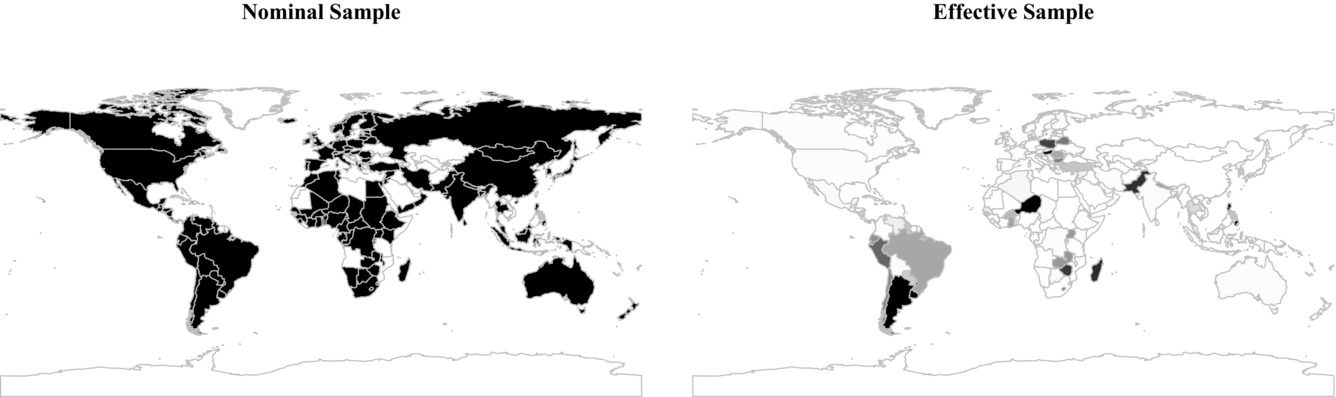
\includegraphics[width = 0.8\textwidth]{figures/arronow_samii_2016.jpeg}
  \end{center}
\end{frame}



\section{More `flexible' approaches and double-robustness}

\begin{frame}{Regression Adjustment and Propensity-scores}
  We have seen two key methods:
  \begin{enumerate}
    \item One relies on estimation of the conditional expectation functions $\mu_d(\bm{x}) = \expec{Y_i}{\bm{X}_i = \bm{x}, D_i = d}$
    
    \item The other relies on estimation of the propensity score $\pi(\bm{x}) = \prob{D_i = 1}{\bm{X}_i = \bm{x}}$
  \end{enumerate}

  \bigskip
  Both will suffer problems if you specify an incorrect functional form (e.g. you incorrectly assume linearity in $\bm{X}_i$)
  \begin{itemize}
    \item This is true even if we have that conditional independence assumption and overlap holding! 
  \end{itemize}
\end{frame}

\begin{frame}{Approach 1}{Machine Learning}
  One thing that folks can do is leverage machine learning methods to more flexibly model $\mu_d(\bm{x})$ and $\pi(\bm{x})$
  \begin{itemize}
    \item Make the models very flexible (polynomials, bins, interactions between $\bm{X}$, etc.)
  \end{itemize}

  However, this runs the risk of over-fitting and creating very noisy (and hence unreliable) estimates

  \pause
  \bigskip
  Machine learning methods (and cross-validation) can be used to prevent overfitting while remaining flexible
  \begin{itemize}
    \item See ``Double/Debiased Machine Learning'' paper in Econometrics Journal for approachable introduction
  \end{itemize}
\end{frame}

\begin{frame}{Approach 2}{Doubly-robust estimators}
  A more traditional approach is to use a \alert{doubly-robust estimator} where you use estimates for both $\mu_d(\bm{x})$ and $\pi(\bm{x})$
  \begin{itemize}
    \item The idea is to have ``2 shots'' at getting it right
  \end{itemize}
\end{frame}

\begin{frame}{Doubly-robust treatment effect estimator}
  The augmented IPW (AIPW) estimator of Robins, Rotnitzky, and Zhao (1994):
  \begin{align*}
    \hat{\tau}_{\texttt{DR}} &= \frac{1}{n} \sum_{i=1}^n \left( \hat{\mu}_{1}(\bm{X}_i) - \hat{\mu}_{1}(\bm{X}_i) \right) \\
    &\quad+ \frac{1}{n} \sum_{i=1}^n \left( 
       \frac{D_i}{\hat{\pi}(\bm{X}_i)} (Y_i - \hat{\mu}_{1}(\bm{X}_i)) -
       \frac{(1 - D_i)}{1 - \hat{\pi}(\bm{X}_i)} (Y_i - \hat{\mu}_{0}(\bm{X}_i)) 
    \right) 
  \end{align*}
  \begin{itemize}
    \item A regression adjustment estimator $+$ an adjustment term
  \end{itemize}
\end{frame}

\begin{frame}{Adjustment term}
  \vspace*{-\bigskipamount}
  $$
    \frac{1}{n} \sum_{i=1}^n \left( 
      \frac{D_i}{\hat{\pi}(\bm{X}_i)} (Y_i - \hat{\mu}_{1}(\bm{X}_i)) -
      \frac{(1 - D_i)}{1 - \hat{\pi}(\bm{X}_i)} (Y_i - \hat{\mu}_{0}(\bm{X}_i)) 
    \right) 
  $$
  The adjustment term $(Y_i - \hat{\mu}_d(\bm{X}_i))$ is the prediction error of our model
  \begin{itemize}
    \item This includes the part of $\mu_d(\bm{X}_i)$ that we failed to estimate
    \item The remaining part biases our treatment effect
  \end{itemize}
  
  Take the prediction error and perform IPW on it to estimate the remaining treatment effect
\end{frame}

\begin{frame}{``Doubly-robust''}
  The AIPW estimator has two great benefits:
  \begin{enumerate}
    \item It is consistent so long as either $\mu_d(\bm{x})$ or $\pi(\bm{x})$ are correctly specified (only 1 is needed, but both is better!)
    
    \pause
    \item If both are correct, then this estimator obtains the `semi-parametric efficiency bound' (as efficient as can be)
  \end{enumerate}

  \pause
  \bigskip
  While theoretically this has great qualities, it is more data hungry
  \begin{itemize}
    \item In smaller finite samples, these estimators can be noisy
  \end{itemize}
\end{frame}

\end{document}
